In large-scale P2P networks, such as the one proposed in this work, peer 
discovery presents a difficult challenge. To better preserve anonymity, nodes 
will have limited knowledge of the network topology and so, the peer discovery 
algorithm was chosen accordingly. Because of the large scale of the network, 
anonymity benefits, robustness, fault tolerance and scalability, the 
\textit{Gossip Algorithm for Peer Discovery based upon Local In-Degree (GPDL)} 
was found to be the right tool for the job. This algorithm uses \textit{Gossip 
Pulling} and \textit{Gossip Pulling} messages to exchange information about 
neighbors between nodes, while maintaining a \textit{Neighbor Table} data 
structure, which stores local topology information \cite{peerdiscovery}.

\begin{figure}
    \centering
    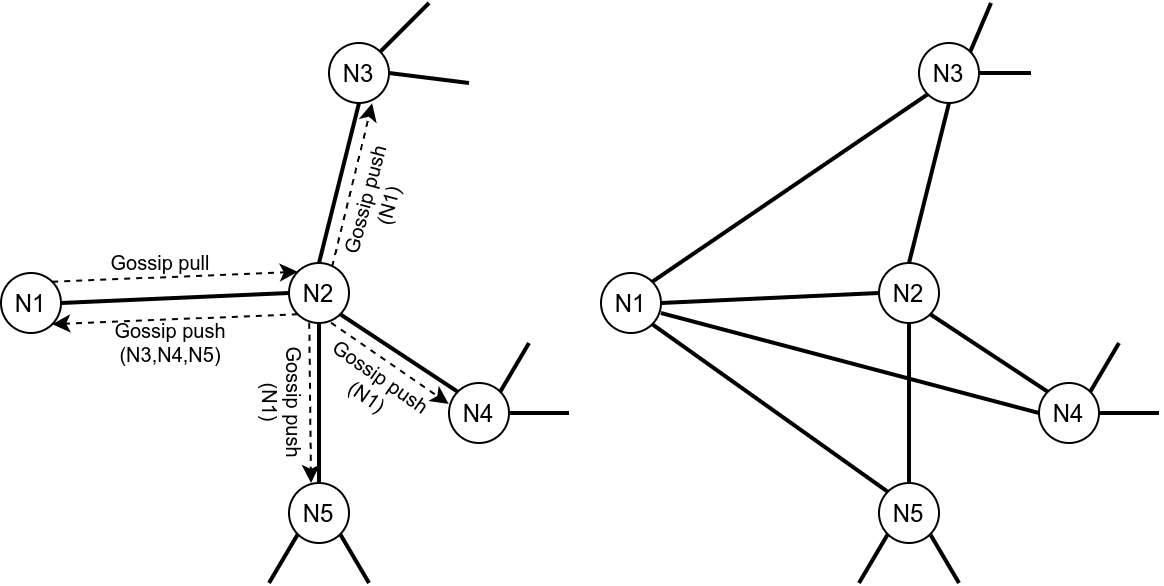
\includegraphics[width=\textwidth]{figures/fig1}
    \caption{Gossip pull and push messages visualization (left). Altered 
network topology after message exchanges (right).}
    \label{fig:fig1}
\end{figure}

It is vital to consider the method by which a new node which joins the networks 
forms the initial list of neighbors. Those will have to be selected from 
various regions or countries to prevent attacks by local adversaries (for 
example those which have access to network information from ISPs). A 
straightforward solution is to have special and publicly known nodes, which 
maintain a list of all the active nodes in the network, called 
\textit{Distributed Node List (DNL)}. Each DNL host will have its own full copy 
of the list of addresses. When a new node joins the network, it will request a 
list of node addresses from one of the DNL hosts, which will arbitrarily select 
them from the list. Besides fulfilling a role for initial node setup, DNL hosts 
can also serve as a background in case all the neighbors of a node go offline. 
When a node leaves the network by closing the client application, it will 
notify one of the DNL hosts, which will them remove the address from the list. 
If a node leaves the network by force, for example if the client crashes, its 
address will still be in the DNL. This is not a severe problem because the DNL 
host can simply ping the addresses before sending them to the node which 
requested them. If one of the addresses belongs to a dead node, then it will 
merely be removed from the list and replaced by another randomly chosen 
address. It is important to note that the DNL hosts are not fully fledged nodes 
in the network, as they will not participate in the usual node discovery and 
file searching algorithms. Plus, they do not have any knowledge about the 
network topology; they just know who are the network participants.

\begin{figure}
    \centering
    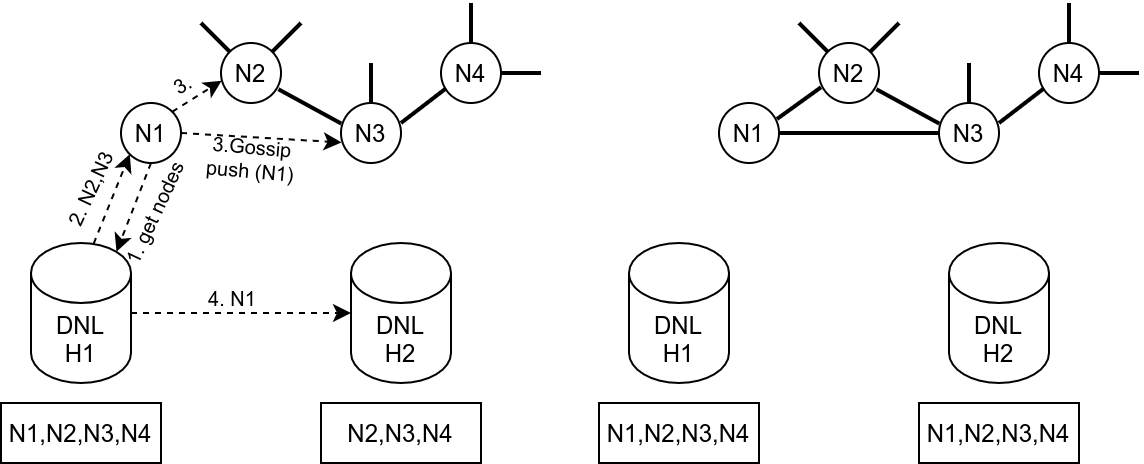
\includegraphics[width=\textwidth]{figures/fig2}
    \caption{Initial setup of a node N1 joining the network. Left: Message 
exchanges. Right: New topology.}
    \label{fig:fig2}
\end{figure}

Full consistency of DNL copies between the DNL hosts is not a requirement and 
differences are completely acceptable. SAND takes advantage of this by 
minimizing the number of synchronization messages between the DNL hosts. 
Instead of sharing every update immediately, changes can be appended to a 
larger message, which is sent less frequently when enough changes are 
accumulated.
